\documentclass[11pt,reqno,final]{amsart}

\pdfcompresslevel=0
\pdfobjcompresslevel=0

\usepackage[dvipsnames]{xcolor}% adds colors
\usepackage{amsmath, amsthm}% {amsfonts, amssymb}

% New Characters
\usepackage[latin1]{inputenc}%
\usepackage[T1]{fontenc}

\usepackage{MnSymbol}
\usepackage[normalem]{ulem}% underlining

\usepackage[theoremfont, largesc]{newpxtext} % different text,math font
\usepackage{newpxmath}

\makeatletter
\DeclareMathRadical{\sqrtsign}{symbols}{112}{largesymbols}{112}
\let\sqrt=\undefined
\DeclareRobustCommand\sqrt{\@ifnextchar[\@sqrt{\mathpalette\@x@sqrt}}
\def\@x@sqrt#1#2{%
 \setbox\z@\hbox{$\m@th#1\sqrtsign{\mkern1mu #2}$}
 \mkern3mu\box\z@}
\makeatother




% Page Typesetting
\usepackage[final]{microtype}
\usepackage{relsize}
\usepackage[margin=1in]{geometry}
\usepackage{framed}
\usepackage{tikz}

\usepackage{hyperref}
\hypersetup{
  final,
  pdftitle={Math 135 - Exp and Log},
  pdfauthor={Bonventre}, 
  linktoc=page,
  pagebackref,
  colorlinks=true,
  citecolor=PineGreen,
  linkcolor=PineGreen,
  linkbordercolor=PineGreen,
}


% Internal References

\usepackage[inline,shortlabels]{enumitem}

\numberwithin{equation}{section} 
\numberwithin{figure}{section}

\usepackage[nameinlink,capitalise,noabbrev]{cleveref}

\crefname{equation}{}{} % get \cref to behave as \eqref

% \theoremstyle{plain} % bold name, italic text
\newtheorem{theorem}[equation]{Theorem}%
\newtheorem*{theorem*}{Theorem}%
\newtheorem{lemma}[equation]{Lemma}%
\newtheorem{proposition}[equation]{Proposition}%
\newtheorem{corollary}[equation]{Corollary}%
\newtheorem{conjecture}[equation]{Conjecture}%
\newtheorem*{conjecture*}{Conjecture}%
\newtheorem{claim}[equation]{Claim}%
\newtheorem{question}{Question}

\theoremstyle{definition} % bold name, plain text
\newtheorem{definition}[equation]{Definition}%
\newtheorem*{definition*}{Definition}%
\newtheorem{example}[equation]{Example}%
\newtheorem*{example*}{Example}%
\newtheorem{remark}[equation]{Remark}%
\newtheorem{notation}[equation]{Notation}%
\newtheorem{convention}[equation]{Convention}%
\newtheorem{assumption}[equation]{Assumption}%
\newtheorem{exercise}[question]{Exercise}

% ---------- macros
\newcommand{\set}[1]{\left\{#1\right\}}%
\newcommand{\sets}[2]{\left\{ #1 \;|\; #2\right\}}%
\newcommand{\longto}{\longrightarrow}%
\newcommand{\into}{\hookrightarrow}%
\newcommand{\onto}{\twoheadrightarrow}%

\usepackage{harpoon}
\newcommand{\vect}[1]{\text{\overrightharp{\ensuremath{#1}}}}

\newcommand{\del}{\partial}%

\newcommand{\ki}{\chi}
\newcommand{\ksi}{\xi}
\newcommand{\Ksi}{\Xi}

% %%%%%%%%%%%%%%%%%%%%%%%%%%%%%%%%%%%%%%%%%%%%%%%%%%%%%%%%%%%%%%%%%%%%%%%%%%%%%%%%%%%%%%%%%%%%%%%%%%%%

\begin{document}

\begin{center}
        \textbf{\Large Math 135, Calculus 1, Fall 2020}\\[10pt]
        {\large 09-14: Exponentials and the Logarithm (Section 1.6)}
\end{center}

\thispagestyle{empty}

\renewcommand{\thesection}{\Alph{section}}

\section{Exponential Functions and the Logarithm}

\textbf{Exponential functions} are of the form $f(x) = b^x$ with $b > 0$.
If $b>1$, $f(x)$ is \textit{increasing}, while if $0<b<1$, $f(x)$ is \textit{decreasing}.
\begin{center}
        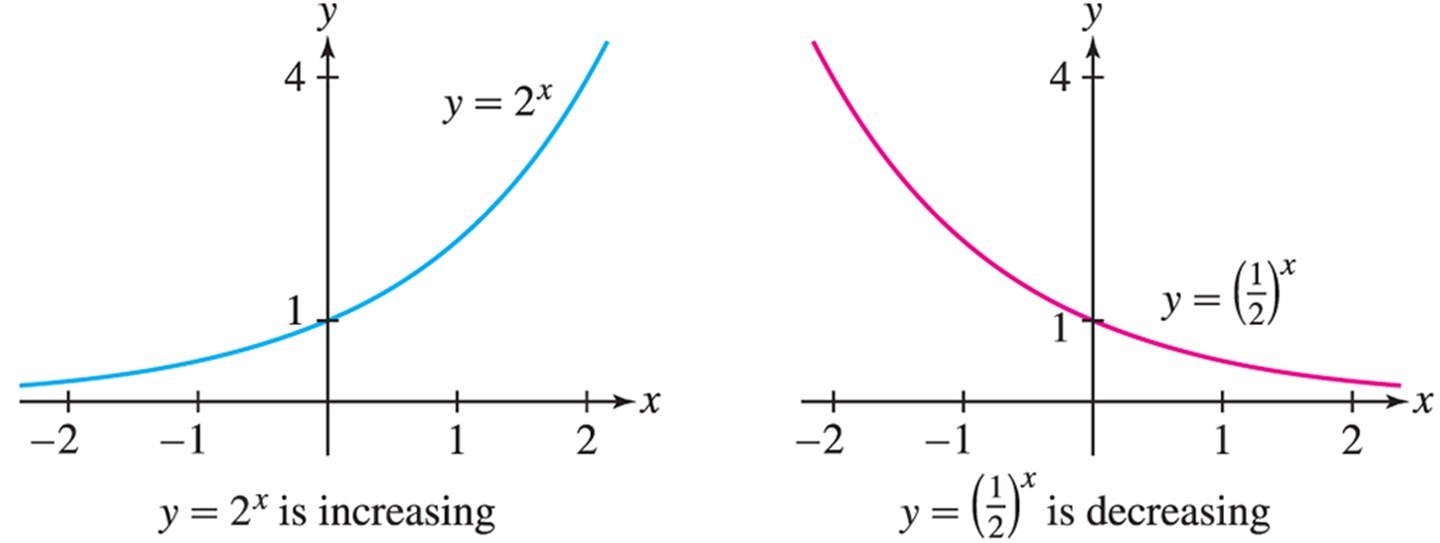
\includegraphics[width=0.8\textwidth]{exp_graphs.png}
\end{center}
Exponential functions are 1-1, so $b^x = b^t$ exactly when $x = t$.

\begin{exercise}
        Suppose $3^{x+1} = \left(\dfrac{1}{3}\right)^{2x}$. Solve for $x$.
        \vfill
\end{exercise}

The \textbf{inverse} of the exponential function $f(x) = b^x$ is called the \textbf{logarithm with base $b$}, denoted $\log_b(x)$.
\begin{center}
        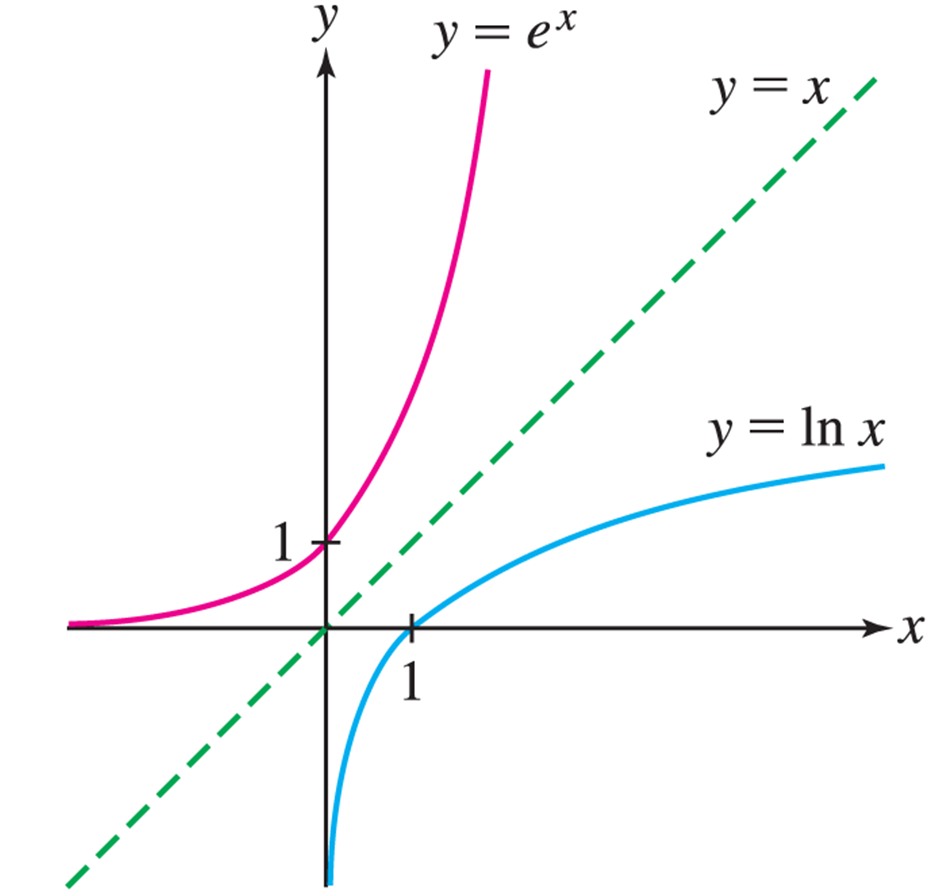
\includegraphics[width=3in]{exp_log_inverse.png}
\end{center}

Using the definition of the inverse, we have:
\begin{framed}
        \[
                y = b^x \quad \mbox{ exactly when } \quad \log_b(y) = x
        \]
\end{framed}

\begin{exercise}
        Use the above to compute $b^{\log_b x}$ and $\log_b(b^x)$.\\
        (Hint: \textbf{inverses!} The answer should not be complicated.)
\end{exercise}

\newpage

\begin{exercise}
        Compute $\log_3(27)$.
        (Hint: let $x = \log_3(27)$. Now apply the above framed box.)
        \vfill
\end{exercise}

\textbf{Euler's number} is the irrational number $e \approx 2.718$.        
The associated exponential $e^x$ has good properties (to be discovered later).
The associated logarithm $\log_e(x) = \ln(x)$ is called the \textbf{natural logarithm}.

\begin{exercise}
        Compute the domain and range of $\ln(x)$.
        \vfill
\end{exercise}

\begin{exercise}
        Use the laws of exponents to compute the following without a calculator; all answers are integers.
        (Hint: use the framed box on the previous page.)        
        \begin{enumerate}[(a)]
        \item $\log_b(1)$ \vfill
        \item $\ln(e)$ \vfill
        \item $\log_6(9) + \log_6(4)$ \vfill
        \end{enumerate}
\end{exercise}

\begin{exercise}
        Suppose a bacteria population doubles in size ever 30 minutes.
        Then, if we started out with 1000 bacteria, we can model this population by the function
        \[
                Q(t) = 1000 \cdot (2)^{t/30}.
        \]
        After how many hours will there be 5000 bacteria?
        \vfill
\end{exercise}

\end{document}




\newpage

